\section{Ngôn ngữ và biểu thức cơ bản trong SageMath}
\subsection{Tổng quan cú pháp và quy tắc trong SageMath}

SageMath sử dụng cú pháp rất giống với Python, nhưng có một số điểm đặc biệt để hỗ trợ tính toán toán học. Dưới đây là một số quy tắc cơ bản mà người dùng cần nắm khi làm việc với SageMath.\\

\subsubsection{Quy tắc chung khi viết lệnh trong SageMath}
\begin{itemize}
	\item \textbf{Biến và tên hàm}: SageMath phân biệt chữ hoa và chữ thường, vì vậy \texttt{x} và \texttt{X} được coi là hai biến khác nhau. Cũng giống như Python, các biến và hàm có thể được sử dụng mà không cần khai báo kiểu dữ liệu.
	
	\item \textbf{Dấu cách}: Dấu cách không ảnh hưởng đến cú pháp trong SageMath, nhưng việc sử dụng dấu cách hợp lý sẽ giúp mã dễ đọc hơn và giảm khả năng xảy ra lỗi.
	
	\item \textbf{Ký tự toán học đặc biệt}: SageMath sử dụng các ký hiệu toán học quen thuộc như \texttt{+} (cộng), \texttt{-} (trừ), \texttt{*} (nhân), \texttt{/} (chia), cùng với nhiều toán tử khác để thực hiện các phép toán.
	
	\item \textbf{Lệnh kết thúc}: Không giống như nhiều ngôn ngữ lập trình khác, SageMath không yêu cầu dấu chấm phẩy (\texttt{;}) để kết thúc lệnh, tuy nhiên bạn vẫn có thể sử dụng dấu đó nếu muốn viết nhiều lệnh trên cùng một dòng.
\end{itemize}



\subsubsection{Cú pháp và quy tắc đặc biệt}

\begin{itemize}
	\item \textbf{Hàm số và đại số}: SageMath cung cấp nhiều hàm tích hợp sẵn để làm việc với biểu thức đại số, bao gồm các hàm lượng giác (\texttt{sin}, \texttt{cos}, \texttt{tan}), hàm mũ (\texttt{exp}), logarit (\texttt{log}), và nhiều hàm toán học khác.
	
	\item \textbf{Đặt tên cho biến}: Việc đặt tên cho biến trong SageMath cần tuân theo các quy tắc sau:
	\begin{itemize}
		\item Tên biến phải bắt đầu bằng một chữ cái (a–z, A–Z) hoặc dấu gạch dưới (\_).
		\item Các ký tự tiếp theo có thể là chữ cái, chữ số (0–9) hoặc dấu gạch dưới.
		\item Không được sử dụng các tên đã được định nghĩa trước trong SageMath, như các từ khóa hoặc tên hàm sẵn có (\texttt{sin}, \texttt{log}, \texttt{var}, \texttt{for}, \texttt{if}, \dots).
	\end{itemize}
\end{itemize}

\subsubsection{Chạy mã trong SageMath}
Để thực thi các lệnh trong SageMath, bạn có thể nhập trực tiếp vào terminal của SageMath hoặc sử dụng môi trường lập trình như Jupyter Notebook. Mã nguồn trong SageMath có thể được viết và lưu vào các file \texttt{.sage} hoặc \texttt{.py}.

Ví dụ về cách chạy một file \texttt{.sage}:

\begin{lstlisting}
	$ sage myscript.sage
\end{lstlisting}

Trong trường hợp bạn sử dụng Jupyter Notebook, bạn có thể chạy từng ô mã (\texttt{cell}) một cách độc lập.

\subsubsection{Quản lý và sử dụng thư viện trong SageMath}
SageMath cung cấp một hệ thống quản lý thư viện mạnh mẽ. Bạn có thể nhập thư viện vào mã của mình để mở rộng chức năng tính toán, ví dụ như nhập các thư viện đại số, giải tích, \dots

Ví dụ nhập thư viện để làm việc với các số nguyên lớn:

\begin{lstlisting}
	sage: from sage.modules.free_module import FreeModule
\end{lstlisting}


\subsection{Biến và kiểu dữ liệu cơ bản}

Trong SageMath, các biến và kiểu dữ liệu cơ bản được sử dụng để thực hiện các phép toán số học, đại số và nhiều phép toán khác. Việc hiểu rõ về các kiểu dữ liệu này là rất quan trọng khi làm việc với SageMath. Dưới đây là các kiểu dữ liệu cơ bản mà bạn sẽ gặp phải khi sử dụng SageMath.

\subsubsection{Khai báo và sử dụng biến}

Biến trong SageMath có thể được khai báo trực tiếp bằng cách gán giá trị cho chúng. SageMath hỗ trợ nhiều loại dữ liệu khác nhau, và bạn không cần phải chỉ định kiểu dữ liệu khi khai báo biến.

Ví dụ:

\begin{lstlisting}
	sage: x = 10  # Bien x la mot so nguyen
	sage: y = 3.14  # Bien y la mot so thuc
	sage: z = "SageMath"  # Bien z la mot chuoi
\end{lstlisting}

Ở trên, chúng ta đã khai báo ba biến với ba kiểu dữ liệu khác nhau:
\begin{itemize}
	\item \texttt{x} là số nguyên (\texttt{integer}),
	\item \texttt{y} là số thực (\texttt{float}),
	\item \texttt{z} là chuỗi ký tự (\texttt{string}).
\end{itemize}
\subsubsection{Kiểu dữ liệu cơ bản trong SageMath}

SageMath hỗ trợ một số kiểu dữ liệu cơ bản, bao gồm:

\begin{itemize}
	\item Số nguyên: Các số nguyên trong SageMath có thể có giá trị âm, dương hoặc bằng không.
	\item Số thực: Là các số có phần thập phân, được sử dụng để làm việc với các phép toán liên quan đến số học.
	\item Chuỗi: Là một chuỗi các ký tự, thường được sử dụng để lưu trữ văn bản.
	\item Danh sách: Là một kiểu dữ liệu để lưu trữ các giá trị trong một dãy. Các giá trị có thể là bất kỳ kiểu dữ liệu nào.
	\item Boolean: Kiểu dữ liệu Boolean có hai giá trị là \texttt{True} và \texttt{False}.
	\item Ma trận và vector: Được sử dụng để làm việc với đại số tuyến tính.
	\item Số nguyên lớn: SageMath hỗ trợ số nguyên có kích thước lớn hơn nhiều so với kiểu dữ liệu chuẩn của Python.
\end{itemize}

\subsubsection{Ví dụ về các kiểu dữ liệu trong SageMath}

Dưới đây là một số ví dụ về cách sử dụng các kiểu dữ liệu cơ bản trong SageMath.

\begin{lstlisting}
	sage: a = 15  # So nguyen
	sage: b = 3.5  # So thuc
	sage: c = "Hello, Sage!"  # Chuoi
	sage: lst = [1, 2, 3, 4, 5]  # Danh sach
	sage: flag = True  # Boolean
\end{lstlisting}

\subsubsection{Chuyển đổi giữa các kiểu dữ liệu}

SageMath cho phép bạn chuyển đổi giữa các kiểu dữ liệu khác nhau một cách dễ dàng.

Ví dụ, bạn có thể chuyển một số thực thành số nguyên:

\begin{lstlisting}
	sage: a = 5.7
	sage: int(a)  # Chuyen doi thanh so nguyen
	5
\end{lstlisting}

Hoặc chuyển đổi một chuỗi thành danh sách các ký tự:

\begin{lstlisting}
	sage: s = "Sage"
	sage: list(s)  # Chuyen doi thanh danh sach ki tu
	['S', 'a', 'g', 'e']
\end{lstlisting}

\subsubsection{Cách làm việc với các tập hợp}

SageMath cũng hỗ trợ kiểu dữ liệu tập hợp, cho phép bạn thực hiện các phép toán trên các tập hợp. Dưới đây là ví dụ về cách tạo và thao tác với tập hợp trong SageMath.

\begin{lstlisting}
	sage: A = Set([1, 2, 3, 4])
	sage: B = Set([3, 4, 5, 6])
	sage: A.union(B)  # Phep hop
	Set([1, 2, 3, 4, 5, 6])
	sage: A.intersubsection(B)  # Phep giao
	Set([3, 4])
\end{lstlisting}

\subsubsection{Thao tác với các số nguyên lớn}

Một trong những tính năng mạnh mẽ của SageMath là khả năng làm việc với các số nguyên lớn. Bạn có thể khai báo và thao tác với các số nguyên có giá trị cực kỳ lớn mà không gặp phải giới hạn như trong các ngôn ngữ lập trình khác.

Ví dụ:

\begin{lstlisting}
	sage: big_number = 123456789123456789123456789
	sage: big_number * 2  # Phep nhan voi mot so lon
	246913578246913578246913578
\end{lstlisting}

\subsection{Lệnh \texttt{show()} trong SageMath}

Lệnh \texttt{show()} trong SageMath dùng để hiển thị biểu thức, kết quả tính toán và trực quan hóa đồ thị dưới dạng ký hiệu toán học đẹp mắt.

\subsubsection{Hiển thị biểu thức toán học}

Lệnh \texttt{show()} giúp biểu diễn kết quả dưới dạng ký hiệu thay vì dạng văn bản thông thường.

\begin{lstlisting}
	# Hien thi bieu thuc
	sage: var('x')
	sage: f = x^2 + 2*x + 1
	sage: show(f)
\end{lstlisting}
	$$x^2 + 2x + 1$$

\subsubsection{Hiển thị đồ thị}

Lệnh \texttt{show()} được sử dụng để vẽ và hiển thị các đồ thị trong không gian 2D và 3D.

\begin{lstlisting}
	# Ve do thi ham so
	sage: plot(x^2, (x, -2, 2)).show()
\end{lstlisting}
\begin{figure}[H]
	\centering
	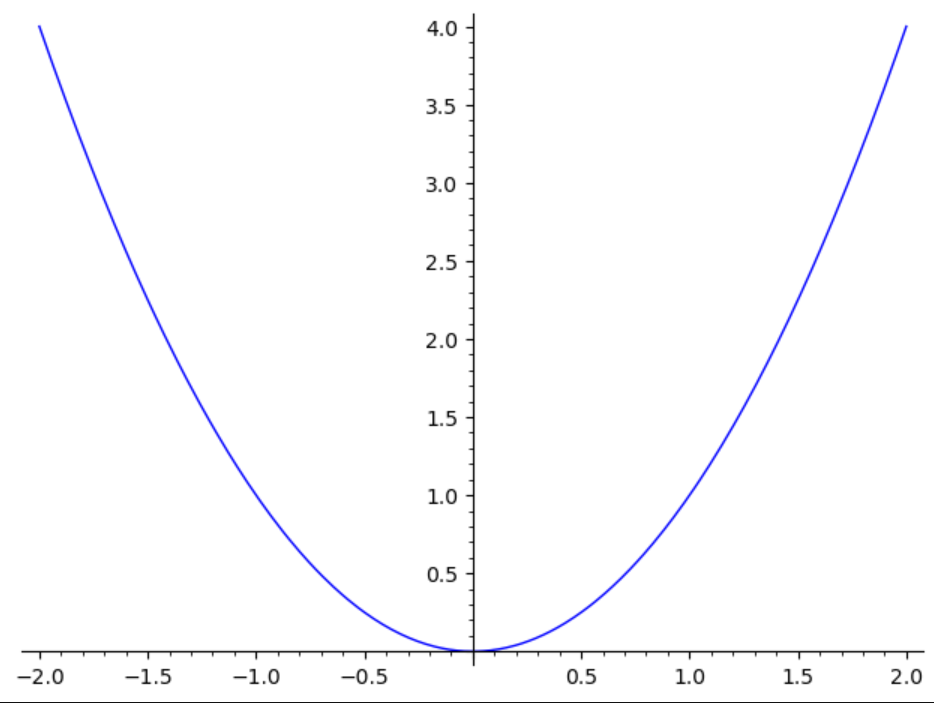
\includegraphics[width=0.7\linewidth]{images/screenshot007}
	\caption{Đồ thị hàm số $y=x^2$ trên đoạn $\left[-2,2\right]$}
	\label{fig:screenshot007}
\end{figure}

\subsubsection{Hiển thị ma trận}

\begin{lstlisting}
	# Hien thi ma tran
	sage: M = matrix([[1, 2], [3, 4]])
	sage: show(M)
\end{lstlisting}
$$\displaystyle \left(\begin{array}{rr}
	1 & 2 \\
	3 & 4
\end{array}\right)$$

Lệnh \texttt{show()} rất hữu ích khi cần trực quan hóa kết quả và trình bày các phép toán.

\subsection{Các phép toán số học và đại số cơ bản}

SageMath hỗ trợ một loạt các phép toán số học và đại số cơ bản, giúp người dùng thực hiện các phép toán cơ bản trong toán học như cộng, trừ, nhân, chia, và các phép toán đại số với các đối tượng phức tạp hơn như đa thức, số nguyên lớn, và các phép toán với các trường số học khác. Dưới đây là các phép toán cơ bản mà bạn sẽ sử dụng thường xuyên trong SageMath.

\subsubsection{Các phép toán số học cơ bản}

SageMath hỗ trợ các phép toán số học thông thường như cộng, trừ, nhân, chia, lũy thừa. Các phép toán này có thể được thực hiện trực tiếp trên các số nguyên, số thực hoặc các đối tượng số học khác.

Ví dụ về phép toán số học cơ bản:

\begin{lstlisting}
	sage: a = 10  # Phep gan
	sage: b = 5  # Phep gan
	sage: a + b  # Cong
	15
	sage: a - b  # Tru
	5
	sage: a * b  # Nhan
	50
	sage: a / b  # Chia
	2.0
	sage: a^b  # Luy thua
	100000
\end{lstlisting}

\subsubsection{Các phép toán với số nguyên lớn}

SageMath hỗ trợ làm việc với các số nguyên có độ dài lớn, vượt quá giới hạn của các kiểu dữ liệu số nguyên trong các ngôn ngữ lập trình khác. Điều này đặc biệt hữu ích khi làm việc với các bài toán lý thuyết số, mã hóa, và mật mã học.

Ví dụ:

\begin{lstlisting}
	sage: big_num = 123456789123456789123456789
	sage: big_num + 1000  # Phep cong voi so lon
	123456789123456789123457789
	sage: big_num * 1000000  # Phep nhan voi so lon
	123456789123456789123456789000000
\end{lstlisting}

\subsubsection{Các phép toán với đa thức}

SageMath hỗ trợ đầy đủ các phép toán đại số với đa thức, bao gồm cộng, trừ, nhân, chia, và các phép toán khác. Để làm việc với đa thức, bạn có thể sử dụng các hàm có sẵn trong SageMath như \texttt{PolynomialRing}.

Ví dụ về các phép toán với đa thức:

\begin{lstlisting}
	sage: R.<x> = PolynomialRing(QQ)  # Khai bao da thuc voi bien x
	sage: f = x^2 + 2*x + 1  # Da thuc f(x) = x^2 + 2x + 1
	sage: g = x^2 - 1  # Da thuc g(x) = x^2 - 1
	sage: f + g  # Cong hai da thuc
	x^2 + 2*x + 1 + x^2 - 1
	sage: f * g  # Nhan hai da thuc
	x^4 + 2*x^3 - x^2 - 2*x - 1
	sage: f / g  # Chia hai da thuc
	(x^2 + 2*x + 1)/(x^2 - 1)
\end{lstlisting}

\subsubsection{Phép chia lấy dư}

SageMath hỗ trợ phép chia lấy dư, cho phép bạn chia hai số nguyên và trả về thương và số dư. Điều này rất hữu ích trong lý thuyết số, đặc biệt là khi làm việc với các thuật toán như thuật toán Euclid.

Ví dụ về phép chia dư:

\begin{lstlisting}
	sage: a = 17
	sage: b = 5
	sage: divmod(a, b)  # Chia du giua 17 va 5
	(3, 2)  # (Thuong, So du)
\end{lstlisting}

\subsubsection{Các phép toán đại số cơ bản}

SageMath không chỉ hỗ trợ các phép toán số học cơ bản mà còn hỗ trợ các phép toán đại số với các đối tượng trừu tượng như nhóm, vành và trường.

Ví dụ về các phép toán nhóm:

\begin{lstlisting}
	sage: G = SymmetricGroup(3)  # Nhom doi xung S3
	sage: G[1] * G[2]  # Nhan hai phan tu trong nhom
	(1, 2)(3)
\end{lstlisting}

\subsubsection{Phép toán lũy thừa}

SageMath hỗ trợ các phép toán lũy thừa với các số nguyên, số thực và các đối tượng đại số. Phép toán lũy thừa có thể được thực hiện bằng ký hiệu mũ \texttt{\^} hoặc dùng hàm \texttt{pow()} (Hàm có sẵn trong ngôn ngữ Python).

Ví dụ về lũy thừa:

\begin{lstlisting}
	# Luy thua so nguyen
	sage: 2^5
	32
	
	# Cach khac su dung hai dau sao
	sage: 2**5
	32
	
	# Luy thua so thuc
	sage: 3.5^2
	12.25
	
	# Cach khac voi so thuc
	sage: pow(3.5, 2)
	12.25
\end{lstlisting}

\textbf{Lưu ý:} Ký hiệu \texttt{**} tương tự như \texttt{\^} để tính lũy thừa, nhưng trong một số trường hợp, \texttt{**} được ưu tiên hơn để tránh lỗi cú pháp.


\section{Đại số, giải tích và hình học}
\subsection{Làm việc với phương trình và hệ phương trình}

Trong SageMath, bạn có thể giải các phương trình đại số đơn giản đến phức tạp, bao gồm phương trình bậc một, bậc hai, và hệ phương trình đại số. SageMath cung cấp các công cụ mạnh mẽ để giải phương trình với một biến hoặc nhiều biến, đồng thời hỗ trợ các phương trình với các hệ số phức tạp.

\subsubsection{Giải phương trình đơn biến}

Để giải một phương trìnhn, bạn có thể sử dụng hàm \texttt{solve()}, nơi đầu vào là phương trình cần giải.

Ví dụ về giải phương trình bậc nhất một ẩn:

\begin{lstlisting}
	sage: x = var('x')  # Dinh nghia bien x
	sage: solve(x + 5 == 0, x)  # Giai phuong trinh x + 5 = 0
	[x == -5]
\end{lstlisting}

SageMath trả về kết quả dưới dạng danh sách các nghiệm. Trong ví dụ trên, phương trình \(x + 5 = 0\) có nghiệm \(x = -5\).

Ví dụ về giải phương trình bậc hai:

\begin{lstlisting}
	sage: solve(x^2 + 5*x + 6 == 0, x)  # Giai phuong trinh bac hai x^2 + 5x + 6 = 0
	[x == -3, x == -2]
\end{lstlisting}

Phương trình bậc hai \(x^2 + 5x + 6 = 0\) có hai nghiệm là \(x = -2\) và \(x = -3\).

\subsubsection{Giải phương trình đa biến}

SageMath cũng hỗ trợ giải các phương trình có nhiều biến. Bạn có thể định nghĩa nhiều biến và sử dụng hàm \texttt{solve()} để giải các hệ phương trình.

Ví dụ về giải hệ phương trình với hai biến:

\begin{lstlisting}
	sage: y = var('y')  # Dinh nghia them bien y
	sage: solve([x + y == 3, x - y == 1], x, y)  # Giai he phuong trinh x + y = 3 va x - y = 1
	[x == 2, y == 1]
\end{lstlisting}

Kết quả là hệ phương trình có nghiệm \(x = 2\) và \(y = 1\).

\subsubsection{Giải phương trình với các hệ số phức tạp}

SageMath cũng cho phép bạn giải các phương trình với các hệ số phức tạp, bao gồm số phức hoặc các biểu thức đại số phức tạp.

Ví dụ về giải phương trình với số phức:

\begin{lstlisting}
	sage: z = var('z', domain=CC)  # Dinh nghia bien Z trong tap so phuc
	sage: solve(z^2 + 1 == 0, z)  # Giai phuong trinh z^2 + 1 = 0 trong tap so phuc
	[z == -I, z == I]
\end{lstlisting}

Phương trình \(z^2 + 1 = 0\) có hai nghiệm là \(z = i\) và \(z = -i\), với \(i\) là đơn vị ảo.

\subsubsection{Giải hệ phương trình đại số phi tuyến}

SageMath cũng hỗ trợ giải các hệ phương trình đại số phi tuyến, bao gồm các phương trình bậc cao hoặc các phương trình có hàm số phi tuyến.

Ví dụ về hệ phương trình phi tuyến:

\begin{lstlisting}
	sage: solve([x^2 + y^2 == 1, x^2 - y^2 == 0], x, y)  # Giai he phuong trinh phi tuyen
	[x == sqrt(2)/2, y == sqrt(2)/2]
\end{lstlisting}

Hệ phương trình đại số phi tuyến \(x^2 + y^2 = 1\) và \(x^2 - y = 0\) có nghiệm \(x = \frac{\sqrt{2}}{2}\) và \(y = \frac{\sqrt{2}}{2}\).

\subsubsection{Sử dụng phương trình trong các bài toán ứng dụng}

SageMath không chỉ giải các phương trình đơn giản mà còn được sử dụng để giải các phương trình trong các bài toán ứng dụng. Bạn có thể sử dụng phương trình để mô hình hóa các bài toán trong các lĩnh vực như vật lý, kỹ thuật, kinh tế học, và khoa học máy tính.

Ví dụ về bài toán mô phỏng sự rơi tự do của vật thể:

\begin{lstlisting}
	sage: t = var('t')  # Dinh nghia bien thoi gian t
	sage: h = 100 - 5*t^2  # Phuong trinh mo ta chieu cao cua vat the theo thoi gian t
	solve(h == 0, t)  # Tim thoi gian vat the cham dat (khi h = 0)
	[t == -2*sqrt(5), t == 2*sqrt(5)]
\end{lstlisting}

Kết quả là \(t = \sqrt{20}\), nghĩa là vật thể chạm đất sau khoảng 4.47 giây.


\subsection{Tính toán đại số trừu tượng (nhóm, vành, trường, đa thức)}

SageMath cung cấp các công cụ mạnh mẽ để làm việc với đại số trừu tượng, bao gồm các cấu trúc đại số cơ bản như vành, nhóm, trường và các phép toán với đa thức. Các cấu trúc này đóng vai trò quan trọng trong các bài toán toán học, vật lý và khoa học máy tính.

\subsubsection{Làm việc với nhóm}

Nhóm là một tập hợp các phần tử với một phép toán nhị phân thỏa mãn các tính chất: đóng, có phần tử trung tính, mỗi phần tử có phần tử nghịch đảo.

Ví dụ về nhóm phép cộng trên các số nguyên modulo 7:

\begin{lstlisting}
	sage: G = Group([1, 2, 3, 4, 5, 6], operation='addition mod 7')  # Nhom cac so nguyen modulo voi phep cong
	sage: G.is_group()  # Kiem tra G co la 1 nhom khong
	True
\end{lstlisting}

Phép toán `operation='addition mod 7'` xác định phép cộng trong nhóm modulo 7. SageMath cung cấp phương thức \texttt{is\_group()} để kiểm tra xem tập hợp có là một nhóm không.

\subsubsection{Làm việc với vành}

Vành là một cấu trúc đại số có hai phép toán: cộng và nhân, và phải thỏa mãn một số tính chất nhất định. Ví dụ về vành các số nguyên modulo 7:

\begin{lstlisting}
	sage: R = Ring([0, 1, 2, 3, 4, 5, 6], addition='mod 7', multiplication='mod 7')  # Vanh cac so nguyen modulo 7
	sage: R.is_ring()  # Kiem tra R co la 1 vanh khong
	True
\end{lstlisting}

Trong ví dụ này, ta tạo ra một vành với phép cộng và phép nhân là phép toán modulo 7.

\subsubsection{Làm việc với trường}

Trường là một cấu trúc đại số trong đó các phép toán cộng, trừ, nhân và chia đều được xác định và có tính nghịch đảo. Trường phổ biến nhất là trường số thực và số phức.

Ví dụ về trường số thực:

\begin{lstlisting}
	sage: F = RealField()  # Tao truong so thuc
	sage: F.is_field()  # Kiem tra F co la 1 truong khong
	True
\end{lstlisting}

SageMath cũng hỗ trợ các trường hữu hạn. Ví dụ về trường hữu hạn:

\begin{lstlisting}
	sage: GF(7)  # Truong huu han F_7
	GF(7)
\end{lstlisting}

Trường này bao gồm các phần tử \{0, 1, 2, 3, 4, 5, 6\}, và các phép toán cộng, nhân, chia đều được thực hiện modulo 7.

\subsubsection{Làm việc với đa thức}

SageMath cung cấp các công cụ mạnh mẽ để làm việc với đa thức, từ các phép toán cơ bản đến các phép toán phức tạp. Bạn có thể thực hiện cộng, trừ, nhân, chia đa thức, giải phương trình đa thức, và làm việc với các đa thức trong các trường hoặc vành.

Ví dụ về tạo đa thức trong một biến:

\begin{lstlisting}
	sage: R.<x> = PolynomialRing(ZZ)  # Tao da thuc trong vanh da thuc co he so nguyen
	sage: p = x^2 + 2*x + 1  # Dinh nghia da thuc
	sage: p.factor()  # Phan tich da thuc thanh nhan tu
	(x + 1)^2
\end{lstlisting}

SageMath phân tích đa thức \(x^2 + 2x + 1\) thành \((x + 1)^2\), điều này giúp ích trong việc giải các phương trình đa thức.

Ví dụ về chia đa thức:

\begin{lstlisting}
	sage: q, r = (x^3 + 2*x^2 + x + 1).div(x^2 + x)  # Chia da thuc
	sage: q, r  # Thuong va phan du
	(x + 1, 1)
\end{lstlisting}

Ở đây, \(x^3 + 2x^2 + x + 1\) chia cho \(x^2 + x\) có thương là \(x + 1\) và phần dư là 1.

\subsubsection{Làm việc với vành đa thức}

Trong SageMath, bạn có thể làm việc với các vành đa thức, nơi phép cộng và nhân được xác định trên các đa thức.

Ví dụ về vành đa thức:

\begin{lstlisting}
	sage: R.<x> = PolynomialRing(ZZ, 'x')  # Vanh cac da thuc voi he so la so nguyen
	sage: I = ideal(x^2 + 1, R)  # Dinh nghia mien cua vanh da thuc
	sage: I.is_ideal()  # Kiem tra I co la mot ideal khong
	True
\end{lstlisting}


\subsection{Ma trận, vector và đại số tuyến tính}

SageMath cung cấp các công cụ mạnh mẽ để làm việc với ma trận, vector và thực hiện các phép toán đại số tuyến tính. Các phép toán này rất quan trọng trong các lĩnh vực như học máy, kỹ thuật, khoa học dữ liệu, và các nghiên cứu toán học.

\subsubsection{Làm việc với vector}

Vector là các đối tượng có thể đại diện cho các điểm trong không gian hoặc các phép toán đại số tuyến tính. Trong SageMath, vector có thể được định nghĩa trong các không gian số học khác nhau như \(\mathbb{R}^n\) hoặc \(\mathbb{C}^n\).

Ví dụ tạo một vector trong không gian thực:

\begin{lstlisting}
	sage: v = vector([1, 2, 3])  # Vector trong khong gian R^3
	sage: v
	(1, 2, 3)
\end{lstlisting}

Bạn có thể thực hiện các phép toán cơ bản trên vector như cộng, trừ, nhân với một số vô hướng (scalar), và tính độ dài:

\begin{lstlisting}
	sage: v + vector([4, 5, 6])  # Cong vector
	(5, 7, 9)
	sage: v * 2  # Nhan vector voi mot so vo huong
	(2, 4, 6)
	sage: v.norm()  # Tinh do dai cua vector
	3.7416573867739413
\end{lstlisting}

Ngoài các phép toán cơ bản, bạn cũng có thể tính tích vô hướng và tích có hướng của các vector. 

Tích vô hướng của hai vector là một phép toán trả về một số vô hướng, được tính bằng tổng các tích của các thành phần tương ứng của hai vector. Ví dụ:

\begin{lstlisting}
	sage: u = vector([1, 2, 3])
	sage: w = vector([4, 5, 6])
	sage: u.dot_product(w)  # Tich vo huong
	32
\end{lstlisting}

Tích có hướng (hoặc tích chéo) là một phép toán giữa hai vector trong không gian ba chiều, cho ra một vector vuông góc với cả hai vector ban đầu. Ví dụ:

\begin{lstlisting}
	sage: u.cross_product(w)  # Tich co huong
	(-3, 6, -3)
\end{lstlisting}


\subsubsection{Làm việc với ma trận}

Ma trận là các bảng số học dùng để biểu diễn các hệ phương trình tuyến tính, phép biến đổi tuyến tính, hoặc các phép toán đại số tuyến tính khác. SageMath cho phép bạn dễ dàng tạo ma trận và thực hiện các phép toán trên ma trận như cộng, nhân, tính định thức, và nghịch đảo.

Ví dụ tạo một ma trận và thực hiện phép cộng:

\begin{lstlisting}
	sage: M = Matrix([[1, 2], [3, 4]])  # Ma tran 2x2
	sage: M
	[1 2]
	[3 4]
	sage: M + Matrix([[5, 6], [7, 8]])  # Cong hai ma tran
	[6 8]
	[10 12]
\end{lstlisting}

Phép nhân ma trận:

\begin{lstlisting}
	sage: M * Matrix([[5], [6]])  # Nhan ma tran voi vector
	[17]
	[39]
\end{lstlisting}

Tính định thức của ma trận:

\begin{lstlisting}
	sage: M.det()  # Tinh dinh thuc cua ma tran
	-2
\end{lstlisting}

Tính nghịch đảo của ma trận (nếu có):

\begin{lstlisting}
	sage: M.inv()  # Tinh ma tran nghich dao
	[-2.0  1.0]
	[ 1.5 -0.5]
\end{lstlisting}

\subsubsection{Làm việc với hệ phương trình tuyến tính}

SageMath hỗ trợ giải các hệ phương trình tuyến tính bằng cách sử dụng ma trận. Ví dụ, để giải một hệ phương trình tuyến tính \(A \cdot x = b\), bạn có thể sử dụng phương thức \texttt{solve()}.

Giải hệ phương trình \( \begin{bmatrix} 1 & 2 \\ 3 & 4 \end{bmatrix} \cdot \begin{bmatrix} x_1 \\ x_2 \end{bmatrix} = \begin{bmatrix} 5 \\ 6 \end{bmatrix} \):

\begin{lstlisting}
	sage: A = Matrix([[1, 2], [3, 4]])  # Ma tran he phuong trinh
	sage: b = vector([5, 6])  # Vector ben phai
	sage: A.solve_right(b)  # Giai he phuong trinh
	(0, 1)
\end{lstlisting}

Phương thức \texttt{solve\_right()} trả về nghiệm của hệ phương trình.

\subsubsection{Giá trị riêng và vectơ riêng}

Một trong những phép toán quan trọng trong đại số tuyến tính là tính giá trị riêng và vectơ riêng của ma trận. SageMath cung cấp phương thức \texttt{eigenvalues()} và \texttt{eigenvectors()} để tính toán các giá trị này.

Tính giá trị riêng của ma trận:

\begin{lstlisting}
	sage: M.eigenvalues()  # Tinh gia tri rieng cua ma tran
	[5.0, -0.9999999999999999]
\end{lstlisting}

Tính vectơ riêng của ma trận:

\begin{lstlisting}
	sage: M.eigenvectors()  # Tinh vector rieng cua ma tran
	[(5.0, 1, [(1, 1)]), (-1.0, 1, [(1, -2)])]
\end{lstlisting}

\subsubsection{Các phép toán đại số tuyến tính khác}

SageMath hỗ trợ nhiều phép toán đại số tuyến tính khác như phân rã ma trận, giải các hệ phương trình, và tính toán với không gian vector. Các phương thức khác bao gồm:

- \texttt{row\_space()}, \texttt{column\_space()}: Tính không gian hàng và không gian cột.
- \texttt{rank()}: Tính hạng của ma trận.
- \texttt{eigenvalues()}: Tính giá trị riêng.
- \texttt{svd()}: Phân rã giá trị kỳ dị (Singular Value Decomposition).

Ví dụ tính hạng ma trận:

\begin{lstlisting}
	sage: M.rank()  # Tinh hang cua ma tran
	2
\end{lstlisting}

\subsection{Đạo hàm, tích phân và giải tích}

SageMath hỗ trợ tính toán đạo hàm, tích phân và các phép toán giải tích khác như giải phương trình vi phân, tính toán số học chính xác cao, và làm việc với các hàm số. Phần này sẽ trình bày cách sử dụng các công cụ giải tích cơ bản trong SageMath để giải quyết các bài toán toán học liên quan đến đạo hàm, tích phân và các phép toán tiếp theo.

\subsubsection{Đạo hàm}

Đạo hàm là một trong những phép toán cơ bản trong giải tích. SageMath cung cấp chức năng để tính đạo hàm của các hàm số, bao gồm cả đạo hàm riêng và đạo hàm toàn phần.

Ví dụ tính đạo hàm của hàm số \(f(x) = x^2 + 3x + 5\):

\begin{lstlisting}
	sage: x = var('x')  # Dinh nghia bien x
	sage: f = x^2 + 3*x + 5  # Dinh nghia ham so
	sage: diff(f, x)  # Tinh dao ham cua f theo x
	2*x + 3
\end{lstlisting}

SageMath cũng cho phép tính đạo hàm bậc cao:

\begin{lstlisting}
	sage: diff(f, x, 2)  # Dao ham bac 2 cua f
	2
\end{lstlisting}

\subsubsection{Tích phân}

Tích phân là phép toán cơ bản trong giải tích, được sử dụng để tính diện tích dưới đường cong, thể tích và nhiều ứng dụng khác. SageMath hỗ trợ tính tích phân bất định và tích phân xác định.

Tính tích phân bất định của hàm \(f(x) = x^2 + 3x + 5\):

\begin{lstlisting}
	sage: integrate(f, x)  # Tinh tich phan bat dinh cua f theo x
	x^3/3 + 3*x^2/2 + 5*x
\end{lstlisting}

Tính tích phân xác định của hàm \(f(x) = x^2\) từ \(x = 0\) đến \(x = 1\):

\begin{lstlisting}
	sage: integrate(x^2, (x, 0, 1))  # Tinh tich phan xac dinh cua x^2 tu 0 den 1
	1/3
\end{lstlisting}

\subsubsection{Giải phương trình vi phân}

SageMath cũng hỗ trợ giải phương trình vi phân (ODEs), bao gồm các phương trình vi phân thường và các phương trình vi phân riêng. Dưới đây là ví dụ về cách giải một phương trình vi phân thông qua phương thức \texttt{desolve()}.

Giải phương trình vi phân \(y' = -2y\) với điều kiện ban đầu \(y(0) = 1\):

\begin{lstlisting}
	sage: y = function('y')(x)  # Dinh nghia ham y(x)
	sage: desolve(-2*y, y, ics=[0,1])  # Giai phuong trinh vi phan voi dieu kien ban dau
	exp(-2*x)
\end{lstlisting}

\subsubsection{Tính toán với chuỗi số học}

SageMath cũng có thể tính toán với chuỗi số học (series), bao gồm các chuỗi hội tụ và phân kỳ. Ví dụ tính chuỗi Taylor của hàm \(\sin(x)\) tại \(x = 0\).

\begin{lstlisting}
	sage: taylor(sin(x), x, 0, 5)  # Tinh chuoi Taylor bac 5 cua sin(x) tai x=0
	x - x^3/6 + O(x^5)
\end{lstlisting}

\subsection{Chuỗi, giới hạn và phép tính xấp xỉ}

SageMath cung cấp các công cụ mạnh mẽ để làm việc với chuỗi số học, tính toán giới hạn và thực hiện các phép tính xấp xỉ. Những công cụ này rất hữu ích khi làm việc với các chuỗi hội tụ hoặc phân kỳ, tính toán giới hạn của các hàm số tại một điểm, và áp dụng các phương pháp xấp xỉ trong các bài toán toán học phức tạp.

\subsubsection{Chuỗi số học}

Chuỗi số học trong SageMath được sử dụng để tính toán và phân tích các chuỗi vô hạn. Các chuỗi này có thể hội tụ hoặc phân kỳ, và việc tính toán các giới hạn của chúng là rất quan trọng trong giải tích.

Ví dụ tính chuỗi của hàm số \(f(x) = \frac{1}{n^2}\) từ \(n = 1\) đến \(n = \infty\):

\begin{lstlisting}
	sage: summation(1/n^2, n, 1, infinity)  # Tinh tong cua chuoi 1/n^2 tu n=1 den vo cung
	pi^2/6
\end{lstlisting}

SageMath có thể tính chuỗi vô hạn và xác định tổng của chuỗi hội tụ như trong ví dụ trên.

\subsubsection{Giới hạn của hàm số}

Giới hạn là một trong những công cụ cơ bản trong giải tích, giúp xác định hành vi của một hàm số khi biến số tiến gần đến một giá trị nhất định. SageMath hỗ trợ tính giới hạn của các hàm số tại một điểm.

Ví dụ tính giới hạn của hàm số \(f(x) = \frac{1}{x}\) khi \(x\) tiến đến \(0\):

\begin{lstlisting}
	# Tinh gioi han cua 1/x khi x tien den 0 tu ben phai
	sage: limit(1/x, x=0, dir='plus')
	+Infinity
	
	# Tinh gioi han cua 1/x khi x tien den 0 tu ben trai
	sage: limit(1/x, x=0, dir='minus')
	-Infinity
\end{lstlisting}

SageMath tự động tính toán giới hạn của các hàm số tại các điểm mà hàm có thể hội tụ hoặc phân kỳ.

\subsubsection{Phép tính xấp xỉ}

SageMath cung cấp nhiều phương pháp để tính xấp xỉ các giá trị của các hàm số, đặc biệt hữu ích khi làm việc với các giá trị không thể tính chính xác hoặc khi cần tốc độ tính toán nhanh.

Ví dụ, tính giá trị xấp xỉ của hàm \(\sin(x)\) tại \(x = 1\) với 10 chữ số thập phân:

\begin{lstlisting}
	sage: sin(1).n(digits=10)  # Tinh gia tri xap xi cua sin(1) voi 10 chu so thap phan
	0.8414710000
\end{lstlisting}

SageMath hỗ trợ tính xấp xỉ cho các phép toán phức tạp, giúp tiết kiệm thời gian tính toán khi không cần độ chính xác tuyệt đối.

\subsubsection{Chuyển đổi giữa chuỗi và số thực}

SageMath cho phép chuyển đổi giữa chuỗi số học và các số thực. Điều này rất hữu ích khi làm việc với các chuỗi số học mà bạn muốn tính toán các giá trị thực gần đúng.

Ví dụ, chuyển đổi chuỗi \( \sum_{n=1}^{\infty} \frac{1}{n^2} \) thành giá trị thực:

\begin{lstlisting}
	sage: summation(1/n^2, n, 1, infinity).n()  # Tinh gia tri gan dung cua chuoi
	1.6449340668
\end{lstlisting}

SageMath cho phép bạn dễ dàng chuyển đổi giữa các biểu thức chính xác và các giá trị số học gần đúng, giúp tiện lợi trong tính toán.


\subsection{Làm việc với hàm số và biểu đồ (vẽ đồ thị 2D, 3D)}

SageMath cung cấp các công cụ mạnh mẽ để làm việc với hàm số và vẽ đồ thị, giúp trực quan hóa các kết quả toán học một cách dễ dàng và hiệu quả. Các đồ thị 2D và 3D có thể được tạo ra cho các hàm số, cung cấp cái nhìn sâu sắc về đặc tính và hành vi của hàm.

\subsubsection{Vẽ đồ thị 2D của hàm số}

Để vẽ đồ thị 2D trong SageMath, bạn có thể sử dụng hàm \texttt{plot}, cho phép vẽ đồ thị của một hàm số trên một khoảng xác định. 

Ví dụ vẽ đồ thị của hàm \( f(x) = \sin(x) \) trên đoạn \( [0, 2\pi] \):

\begin{lstlisting}
	sage: plot(sin(x), (x, 0, 2*pi))  # Ve do thi cua sin(x) tu 0 den 2*pi
\end{lstlisting}
\begin{figure}
	\centering
	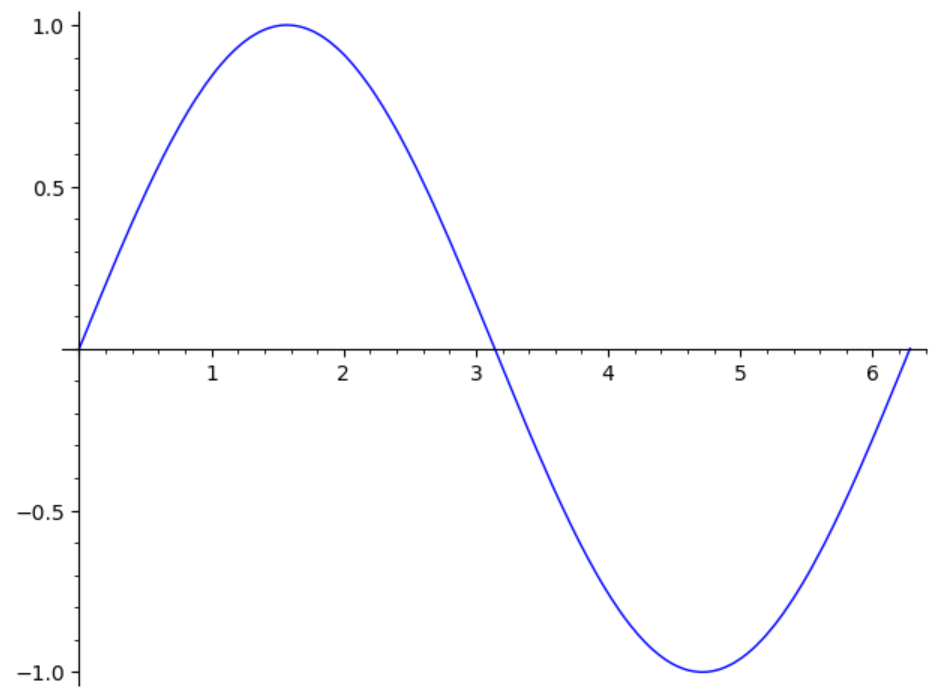
\includegraphics[width=0.7\linewidth]{images/screenshot008}
	\caption{Đồ thị 2D của hàm số \(\sin(x)\) trên đoạn \( [0, 2\pi] \)}
	\label{fig:screenshot008}
\end{figure}

\subsubsection{Vẽ đồ thị 2D của nhiều hàm số}

SageMath hỗ trợ vẽ đồ thị của nhiều hàm số trên cùng một đồ thị. Bạn có thể vẽ nhiều hàm số trên cùng một biểu đồ bằng cách sử dụng toán tử cộng (\(+\)).

Ví dụ, vẽ đồ thị của \( f(x) = \sin(x) \) và \( g(x) = \cos(x) \) trên cùng một đồ thị:

\begin{lstlisting}
	sage: plot(sin(x), (x, 0, 2*pi)) + plot(cos(x), (x, 0, 2*pi))  # Ve dong thoi do thi cua ham sin(x) va cos(x)
\end{lstlisting}
\begin{figure}
	\centering
	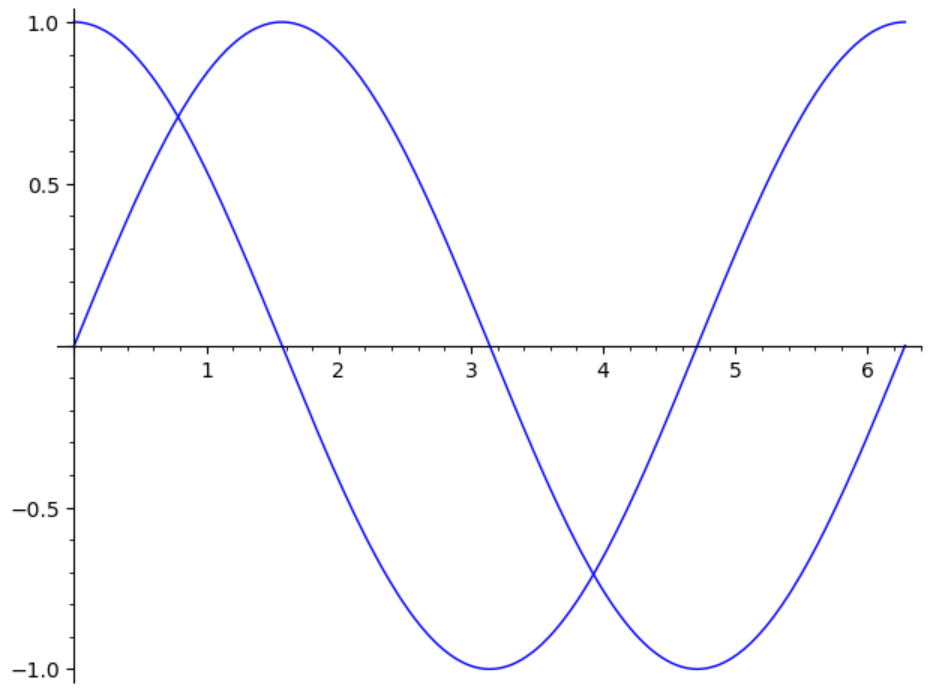
\includegraphics[width=0.5\linewidth]{images/screenshot009}
	\caption{Đồ thị với cả hai hàm \(\sin(x)\) và \(\cos(x)\) trên cùng một biểu đồ}
	\label{fig:screenshot009}
\end{figure}

\subsubsection{Vẽ đồ thị 3D của hàm số}

SageMath cũng cho phép vẽ đồ thị 3D của các hàm hai biến. Để vẽ đồ thị 3D, bạn có thể sử dụng hàm \texttt{plot3d}. Ví dụ, vẽ đồ thị của hàm \( f(x, y) = \sin(x^2 + y^2) \):

\begin{lstlisting}
	sage: plot3d(sin(x^2 + y^2), (x, -3, 3), (y, -3, 3))  # Ve do thi 3D cua ham sin(x^2 + y^2)
\end{lstlisting}
\begin{figure}
	\centering
	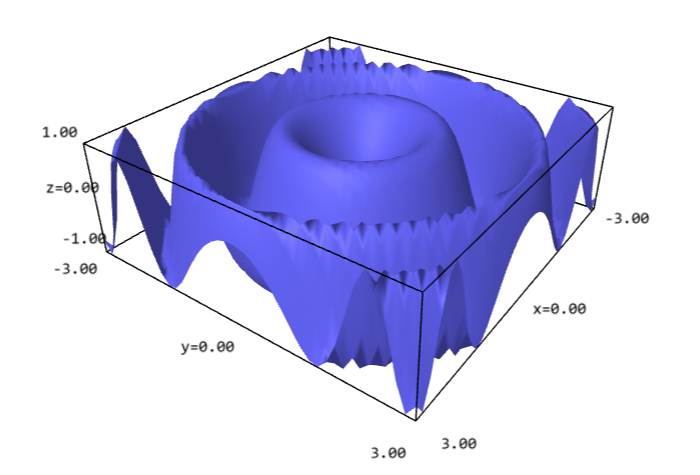
\includegraphics[width=0.7\linewidth]{images/screenshot010}
	\caption{Một bề mặt 3D của hàm \( \sin(x^2 + y^2) \) trong khoảng \([-3, 3]\) cho cả \(x\) và \(y\)}
	\label{fig:screenshot010}
\end{figure}

\subsubsection{Tùy chỉnh đồ thị}

SageMath cung cấp nhiều tùy chọn để tùy chỉnh đồ thị, chẳng hạn như thay đổi màu sắc, thêm tiêu đề, điều chỉnh trục, hoặc thay đổi độ dày đường nét. Các tùy chọn này có thể giúp bạn tạo ra các biểu đồ trực quan và dễ hiểu hơn.

Ví dụ, vẽ đồ thị của hàm \( f(x) = e^x \) và thêm tiêu đề, nhãn trục:

\begin{lstlisting}
	# Ve do thi ham so exp(x) voi tieu de va nhan
	sage: p = plot(exp(x), (x, 0, 5), color='green')
	sage: p.axes_labels(['x', 'exp(x)'])
	sage: p.show(title='Graph of exp(x)')
\end{lstlisting}
\begin{figure}
	\centering
	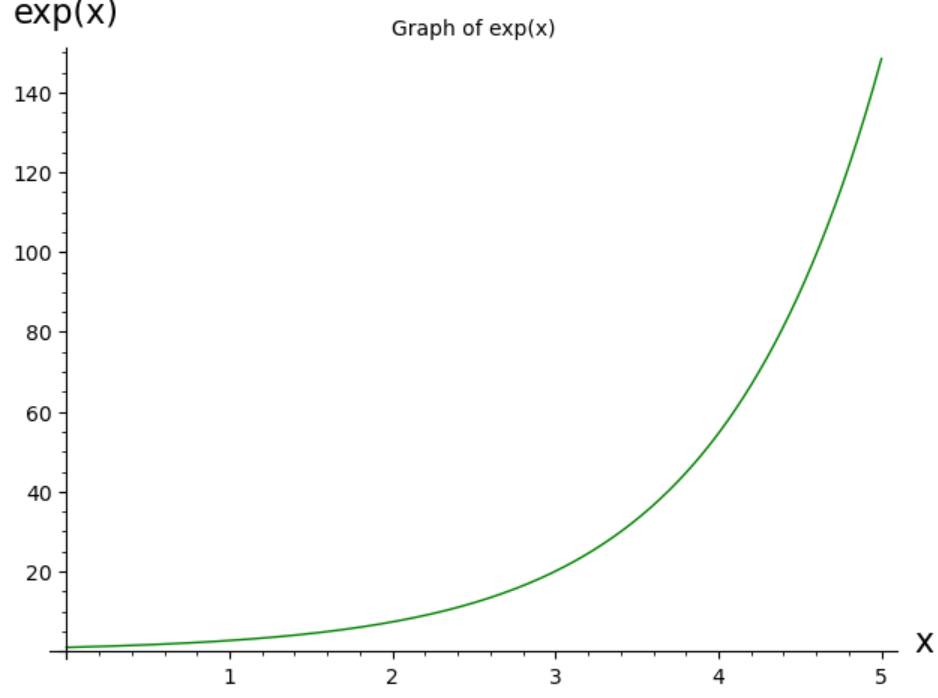
\includegraphics[width=0.7\linewidth]{images/screenshot011}
	\caption{Đồ thị của \( e^x \) với màu xanh lá, thêm tiêu đề cùng với nhãn cho các trục}
	\label{fig:screenshot011}
\end{figure}

\subsubsection{Vẽ đồ thị parametric}

SageMath cũng hỗ trợ vẽ đồ thị các hàm parametric. Các hàm parametric được định nghĩa bởi một cặp hàm số \( x(t) \) và \( y(t) \), với \( t \) là tham số. Ví dụ, vẽ đồ thị của đường tròn với bán kính \(r = 1\):

\begin{lstlisting}
	sage: var('t')	#Khai bao bien t
	sage: parametric_plot([cos(t), sin(t)], (t, 0, 2*pi))  # Ve do thi cua duong tron
\end{lstlisting}
\begin{figure}
	\centering
	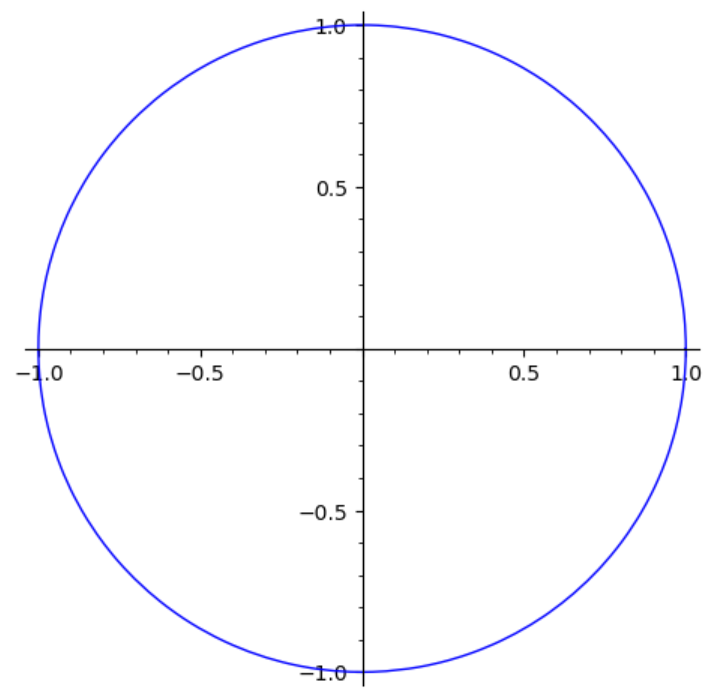
\includegraphics[width=0.7\linewidth]{images/screenshot012}
	\caption{Đồ thị của một đường tròn đơn vị trong mặt phẳng \( Oxy \)}
	\label{fig:screenshot012}
\end{figure}

\section{Tổ hợp, xác suất và logic}
\subsection{Tính toán tổ hợp, xác suất và thống kê}

SageMath cung cấp một bộ công cụ mạnh mẽ để làm việc với các vấn đề tổ hợp, xác suất và thống kê. Phần này sẽ giới thiệu cách sử dụng SageMath để thực hiện các phép toán tổ hợp, tính xác suất và xử lý các bài toán thống kê.

\subsubsection{Tính toán tổ hợp}

Trong tổ hợp, các phép toán như chèn chỗ và kết hợp được sử dụng để tính toán số cách chọn một tập hợp con từ một tập hợp lớn hơn. SageMath cung cấp các hàm như \texttt{binomial} và \texttt{factorial} để tính các giá trị tổ hợp, chỉnh hợp và giai thừa.

Ví dụ, tính số cách chọn 3 phần tử từ một tập hợp 5 phần tử:

\begin{lstlisting}
	sage: binomial(5, 3)  # Tinh to hop chap 3 cua 5
	10
\end{lstlisting}

Ví dụ, tính số cách chọn và sắp xếp 3 phần tử từ một tập hợp 5 phần tử:
\begin{lstlisting}
	sage: permutation(5, 3)  # Tinh chinh hop 3 cua 5
	60
\end{lstlisting}

Ngoài ra, bạn có thể tính giai thừa của một số bằng cách sử dụng hàm \texttt{factorial}:

\begin{lstlisting}
	sage: factorial(5)  # Tinh 5!
	120
\end{lstlisting}

\subsubsection{Tính toán xác suất}

SageMath hỗ trợ tính toán xác suất trong các bài toán tổ hợp. Để tính xác suất, bạn có thể sử dụng các hàm như \texttt{probability}, \texttt{random}, và các hàm xác suất phân phối.

Ví dụ, tính xác suất để một con xúc xắc ra mặt 6:

\begin{lstlisting}
	sage: P = 1/6  # Xac suat ra mat 6
	P
	1/6
\end{lstlisting}

SageMath cung cấp hàm \texttt{probability} để tính toán xác suất trong các bài toán phức tạp hơn, đặc biệt khi làm việc với các phân phối xác suất. Ví dụ, ta có thể tính xác suất của một sự kiện trong một không gian mẫu xác định, chẳng hạn xác suất để lăn xúc xắc và ra mặt 6:

\begin{lstlisting}
	sage: P = probability(lambda: random_integer(1, 6) == 6)  # Xac suat ra mat 6
	P
	1/6
\end{lstlisting}

SageMath cũng hỗ trợ việc tạo các giá trị ngẫu nhiên từ phân phối xác suất. Ví dụ, để tạo một giá trị ngẫu nhiên từ phân phối đồng đều trên khoảng từ 1 đến 6 (giống như lăn xúc xắc), bạn có thể sử dụng hàm \texttt{random\_integer}:

\begin{lstlisting}
	sage: random_integer(1, 6)  # Sinh so ngau nhien giua 1 va 6
\end{lstlisting}

Hàm \texttt{random\_integer(a, b)} sẽ trả về một giá trị ngẫu nhiên trong khoảng từ \(a\) đến \(b\), bao gồm cả \(a\) và \(b\).

Bạn cũng có thể tính xác suất của các sự kiện phức tạp hơn, chẳng hạn như xác suất ra mặt chẵn khi lăn một con xúc xắc. Sử dụng hàm \texttt{probability} với một điều kiện phức tạp:

\begin{lstlisting}
	sage: P_even = probability(lambda: random_integer(1, 6) in [2, 4, 6])  # Xac suat ra mat chan
	P_even
	1/2
\end{lstlisting}

Ở đây, chúng ta đã tính xác suất ra mặt chẵn của con xúc xắc. Kết quả xác suất là \( \frac{3}{6} = \frac{1}{2} \), vì có ba mặt chẵn (2, 4, 6) trong tổng số sáu mặt của xúc xắc.

\subsubsection{Phân phối xác suất}

SageMath hỗ trợ nhiều loại phân phối xác suất, bao gồm phân phối nhị thức, phân phối chuẩn và phân phối Poisson. Bạn có thể sử dụng các hàm như\\ \texttt{binomial\_distribution}, \texttt{normal\_distribution}, và \texttt{poisson\_distribution} để làm việc với các phân phối này.

Ví dụ, tính xác suất để có ít nhất 3 mặt "được" trong 5 lần gieo xúc xắc với phân phối nhị thức:

\begin{lstlisting}
	sage: B = binomial_distribution(5, 1/6)  # Phan phoi nhi thuc cho 5 lan gieo
	P = B.cdf(3)  # Cumulative distribution function de tinh xac suat co it nhat 3 lan "duoc"
	P
	0.868050607
\end{lstlisting}

\subsubsection{Tính toán thống kê}

SageMath cũng cung cấp các công cụ mạnh mẽ để tính toán thống kê mô tả như trung bình, phương sai, độ lệch chuẩn và các phép toán thống kê khác.

Ví dụ, tính trung bình và độ lệch chuẩn của một dãy số:

\begin{lstlisting}
	sage: data = [12, 15, 20, 25, 30, 35, 40]
	sage: mean(data)  # Tinh trung binh
	25.2857142857143
	sage: stdev(data)  # Tinh do lech chuan
	9.49460415914107
\end{lstlisting}

Các hàm \texttt{mean} và \texttt{stdev} tính toán trung bình và độ lệch chuẩn của dãy số.

\subsubsection{Kiểm định giả thuyết}

SageMath cung cấp các công cụ để thực hiện các kiểm định giả thuyết thống kê. Ví dụ, kiểm định t-Student để kiểm tra sự khác biệt giữa trung bình mẫu và trung bình giả thuyết.

Ví dụ, thực hiện kiểm định t với dãy số và trung bình giả thuyết là 25:

\begin{lstlisting}
	sage: t_test(data, 25)  # Kiem dinh t voi trung binh gia thuyet 25
	(0.285714285714286, 0.781595168902066)
\end{lstlisting}

Kết quả trả về là giá trị thống kê t và giá trị p. Với giá trị p này, bạn có thể quyết định có bác bỏ giả thuyết hay không.


\subsection{Làm việc với số học rời rạc và lý thuyết số}

SageMath cung cấp các công cụ rất mạnh mẽ để làm việc với số học rời rạc và lý thuyết số, cho phép thực hiện từ những thao tác đơn giản như tính \texttt{mod}, kiểm tra nguyên tố đến những thao tác phức tạp hơn như định lý phần dư Trung Hoa, logarit rời rạc, và hệ thống số học hữu hạn.

\subsubsection{Số nguyên tố và kiểm tra nguyên tố}

Bạn có thể dễ dàng tạo danh sách các số nguyên tố hoặc kiểm tra một số có phải nguyên tố hay không bằng các hàm \texttt{is\_prime}, \texttt{next\_prime}, \texttt{prime\_pi}, và \texttt{primes}.

\begin{lstlisting}
	sage: is_prime(37)
	True
	sage: next_prime(100)
	101
	sage: primes(50, 70)
	[53, 59, 61, 67]
\end{lstlisting}

\subsubsection{Ước số chung lớn nhất và bội số chung nhỏ nhất}

SageMath hỗ trợ tính ước số chung lớn nhất (GCD) và bội số chung nhỏ nhất (LCM) bằng các hàm \texttt{gcd} và \texttt{lcm}.

\begin{lstlisting}
	sage: gcd(48, 180)
	12
	sage: lcm(12, 18)
	36
\end{lstlisting}

\subsubsection{Số học modulo}

Số học modulo là nền tảng trong nhiều thuật toán lý thuyết số. Bạn có thể sử dụng toán tử \texttt{\%} hoặc tạo trường số dư với \texttt{Zmod(n)}.

\begin{lstlisting}
	sage: 17 % 5
	2
	sage: R = Zmod(7)
	sage: a = R(3)
	sage: b = R(5)
	sage: a * b
	R(1)
\end{lstlisting}

\subsubsection{Định lý phần dư Trung Hoa}

SageMath hỗ trợ định lý phần dư Trung Hoa qua hàm \texttt{crt} để tìm số thỏa mãn một hệ phương trình đồng dư.

\begin{lstlisting}
	sage: crt([2, 3, 2], [3, 5, 7])  # Chinese Remainder Theorem
	23
\end{lstlisting}

\subsubsection{Hàm Euler và số nguyên tố cùng nhau}

Hàm Euler \(\phi(n)\) đếm số nguyên nhỏ hơn \(n\) nguyên tố cùng nhau với \(n\). SageMath cung cấp hàm \texttt{euler\_phi} và \texttt{is\_coprime} để làm việc với tính chất này.

\begin{lstlisting}
	sage: euler_phi(10)
	4
	sage: gcd(7, 10) == 1  # 7 and 10 are coprime
	True
\end{lstlisting}

\subsubsection{Lũy thừa modulo và logarit rời rạc}

Phép toán lũy thừa modulo có thể được thực hiện hiệu quả với hàm \texttt{power\_mod}, và SageMath cũng hỗ trợ tìm logarit rời rạc trong một số trường hợp.

\begin{lstlisting}
	sage: power_mod(3, 4, 5)
	1
	sage: Z5 = Zmod(5)
	sage: Z5(3).log(2)  # Solve 2^x = 3 mod 5
	3
\end{lstlisting}

\subsubsection{Trường số và phần tử đại số}

SageMath cho phép bạn tạo và làm việc với các trường số (number fields), ví dụ trường chứa căn bậc hai hoặc các phần tử đại số khác.

\begin{lstlisting}
	sage: K.<a> = NumberField(x^2 - 2)
	sage: a^2
	2
\end{lstlisting}


\subsection{Tính toán với tập hợp, logic và điều kiện}

SageMath hỗ trợ nhiều công cụ để thao tác với tập hợp, biểu thức logic và điều kiện. Các cấu trúc này không chỉ hữu ích trong toán học rời rạc mà còn trong việc xây dựng mô hình, tự động hóa kiểm định mệnh đề và viết mã có điều kiện.

\subsubsection{Tập hợp và các phép toán trên tập hợp}

Bạn có thể định nghĩa các tập hợp và thực hiện các phép toán như hợp, giao, hiệu, hiệu đối xứng và kiểm tra phần tử.

\begin{lstlisting}
	sage: A = Set([1, 2, 3, 4])
	sage: B = Set([3, 4, 5, 6])
	sage: A.union(B)
	{1, 2, 3, 4, 5, 6}
	sage: A.intersubsection(B)
	{3, 4}
	sage: A.difference(B)
	{1, 2}
	sage: A.symmetric_difference(B)
	{1, 2, 5, 6}
	sage: 3 in A
	True
\end{lstlisting}

Ngoài ra, SageMath còn hỗ trợ tập rỗng, tập vô hạn, tập định nghĩa bằng điều kiện và các tập số học đặc biệt như tập số nguyên, tập số thực, tập hữu tỷ, \dots

\begin{lstlisting}
	sage: EmptySet()
	{}
	sage: QQ.is_subset(RR)
	True
\end{lstlisting}

\subsubsection{Biểu thức logic và phép toán mệnh đề}

SageMath cho phép tạo và đánh giá các biểu thức logic sử dụng các phép toán: \texttt{and}, \texttt{or}, \texttt{not}, \texttt{xor}, \texttt{implies}, \texttt{iff}.

\begin{lstlisting}
	sage: a, b = var('a b')
	sage: f = a & ~b
	sage: f.simplify_logic()
	a & ~b
\end{lstlisting}

Bạn cũng có thể kiểm tra tính đúng sai hoặc tương đương logic giữa các biểu thức.

\begin{lstlisting}
	sage: f1 = (a & b) | (~a & b)
	sage: f2 = b
	sage: bool(f1.simplify_logic() == f2.simplify_logic())
	True
\end{lstlisting}

\subsubsection{Câu lệnh điều kiện \texttt{if} và các biểu thức điều kiện}

Trong khi SageMath chủ yếu dùng cho biểu thức toán học, nó cũng hỗ trợ biểu thức điều kiện trong mã Python:

\begin{lstlisting}
	sage: x = 5
	sage: if x % 2 == 0:
	....:     y = "even"
	....: else:
	....:     y = "odd"
	sage: y
	'odd'
\end{lstlisting}

Bạn có thể dùng biểu thức điều kiện ngắn gọn dạng \texttt{a if condition else b}:

\begin{lstlisting}
	sage: z = "positive" if x > 0 else "non-positive"
	sage: z
	'positive'
\end{lstlisting}

\subsubsection{Mệnh đề định lượng: forall và exists}

Trong SageMath, việc biểu diễn các lượng từ toán học (\texttt{forall}, \texttt{exists}) không được hỗ trợ trực tiếp thông qua các hàm \texttt{ForAll} và \texttt{Exists} như trong một số ngôn ngữ lập trình khác. Thay vào đó, chúng ta có thể sử dụng các phương pháp kiểm tra tính đúng của mệnh đề bằng cách sử dụng các hàm kiểm tra giá trị cụ thể hoặc dùng giả thuyết với hàm \texttt{assume()}.

\textbf{Ví dụ:} Kiểm tra mệnh đề với tập giá trị hữu hạn

\begin{lstlisting}
	# Kiem tra dieu kien x^2 >= 0 voi cac gia tri cu the
	sage: x = var('x')
	sage: all((x^2 >= 0) for x in [-10, -1, 0, 1, 10])
	# Ket qua: True
\end{lstlisting}

\textbf{Ví dụ:} Kiểm tra với giả thuyết

\begin{lstlisting}
	# Kiem tra dieu kien voi gia thuyet x la so thuc
	sage: assume(x, 'real')
	sage: bool(x^2 >= 0)
	# Ket qua: True
\end{lstlisting}
